\documentclass{article}
\usepackage{verbatim}
\usepackage{amsmath}
\usepackage[margin=1in,left=1.5in,includefoot]{geometry}
\usepackage{graphicx}
\usepackage{systeme}
\usepackage{listings}
\usepackage{color}
\usepackage{xcolor}
\usepackage{graphicx}
\usepackage{float}
\usepackage{hyperref}
\usepackage{placeins}
\usepackage{fancyhdr}
\definecolor{mygreen}{RGB}{28,172,0} % color values Red, Green, Blue
\definecolor{mylilas}{RGB}{170,55,241}
\pagestyle{fancy}
\fancyhead{}
\fancyfoot{}
\fancyfoot[R]{ \thepage\ }
\usepackage[utf8]{inputenc}

% Default fixed font does not support bold face
\DeclareFixedFont{\ttb}{T1}{txtt}{bx}{n}{12} % for bold
\DeclareFixedFont{\ttm}{T1}{txtt}{m}{n}{12}  % for normal

% Custom colors
\usepackage{color}
\definecolor{deepblue}{rgb}{0,0,0.5}
\definecolor{deepred}{rgb}{0.6,0,0}
\definecolor{deepgreen}{rgb}{0,0.5,0}


\begin{document}


\begin{titlepage}
  \begin{center}
  \huge{Yujin Liu, Helen Jin, Jiangmeng Li}
  \end{center}


\end{titlepage}


\section{Introduction to the SIR Model and Notation}
The susceptible-infected-removed (SIR) model is built based on the first-order derivative to model the spread of infectious disease, where the time dependent variables $S$, $I$, $R$ each represent the following populations:

$S$(susceptible): number of individuals who are not infected but could become infected

$I$(infected): number of individuals who are already infected and can spread disease

$R$(removed): number of individuals who are either recovered and immune or have died
    
And $s$, $i$, $r$ are used to represent the proportion of susceptible, infected and removed individuals among the population. 

There are two parameters $b$ and $k$ in the model, where $b$ indicates the number of interactions each day that could spread the disease (per individual) and $k$ indicates the fraction of the infectious population which recovers each day. 

In the ODE-based model, we can get the following system of differential equations, where $t$ is time:

$\frac{ds}{dt} = -b * s(t) * i(t)$

$\frac{dr}{dt} = k * i(t)$

$\frac{di}{dt} = b * s(t) * i(t) - k * i(t)$
\section{Python Package 'sir'}


\section{Results of Simulations}
\subsection{Discrete Agent-Based Model}

To investigate how a new disease spreads, we run the simulations of the discrete agent-based model and the continuous ODE model, starting with 100 infectious individuals out of total population 20000. 

We generate several plots to show how s, i, and r change over the length of the simulation for a couple different choices of k and b. First we check the plots for b = 2, which means we assume each individual has two interactions each day that could spread the disease, with different k values. 

\begin{figure}[htp]

\centering
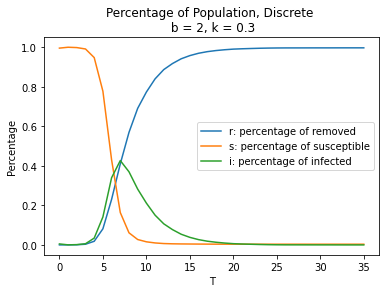
\includegraphics[width=.3\textwidth]{Figure1_discrete_sir_b2_k1.png}\hfill
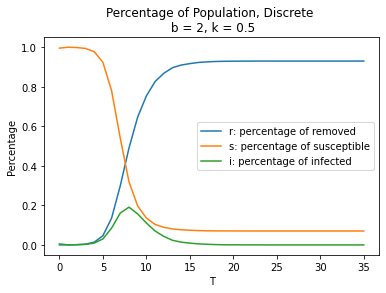
\includegraphics[width=.3\textwidth]{Figure1_discrete_sir_b2_k2.png}\hfill
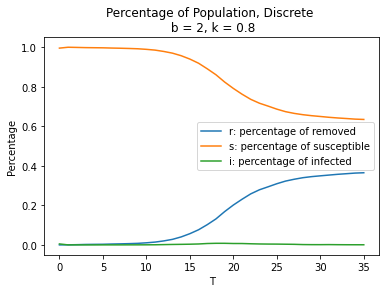
\includegraphics[width=.3\textwidth]{Figure1_discrete_sir_b2_k3.png}

\caption{Percentage of population susceptible (s), infected (i), and removed (r), discrete}
\label{fig:figure3}

\end{figure}



From the plots, we find that when the recovery rate is low (0.3), finally all people are removed, which indicates that all people were infectious and either have recovered and are now immune, or have died. As the recovery rate increases to a high value (0.8), the trends change obviously. The percentage of infected people does not increase, and the percentage of removed people increases to approximately 0.4 while the percentage of susceptible people decreases to 0.6. Finally, both trends of removed and susceptible people stays constant. In this case, there are fairly large proportion of individuals who are never infected. Thus, when the recovery rate k is large enough (larger than 0.6) and b is relatively small (less than 3), then the herd immunity is eventually achieved. The herd immunity occurs when a large portion of a community becomes immune to a disease, making the spread of disease unlikely, so the whole community becomes protected. Next, we increase the value of b and see whether the trends change. 


\begin{figure}[htp]

\centering
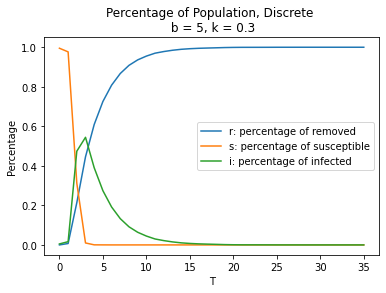
\includegraphics[width=.3\textwidth]{Figure1_discrete_sir_b5_k1.png}\hfill
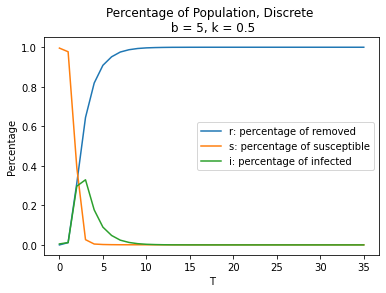
\includegraphics[width=.3\textwidth]{Figure1_discrete_sir_b5_k2.png}\hfill
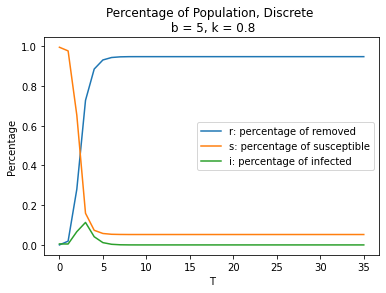
\includegraphics[width=.3\textwidth]{Figure1_discrete_sir_b5_k3.png}

\caption{Percentage of population susceptible (s), infected (i), and removed (r), discrete}
\label{fig:figure3}

\end{figure}



When b = 5, each individual has five interactions each day that could spread the disease. These plots suggest that when each individual get contacts with five infectious people per day, if the recovery rate is 0.3, then finally all people are removed after 20 days; if the recovery rate is 0.5, all people are removed after 10 days; even if the recovery rate is 0.8, less than 10 percent of individuals will remain susceptible after 10 days. As a result, when b is large enough, no matter how large k is, almost all people will be removed eventually, which means that all people will be infected and left with different results. Hence, people should avoid contacting in person with infectious people. Some suggestions include staying at home as much as possible and avoiding visiting areas where the disease is prevalent. 


Now, we want to investigate some qualitative behaviors of the simulations based on the parameters b and k in the phase diagrams. 
The simulations are done with T values 10, 20 and 30 days for both discrete and continuous cases. 


\begin{figure}[htp]

\centering
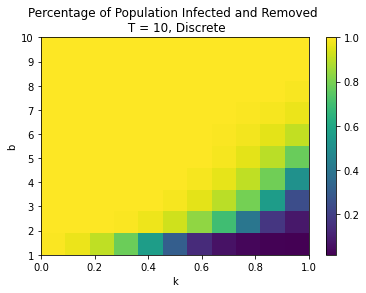
\includegraphics[width=.3\textwidth]{Figure1_discrete_diagT10total.png}\hfill
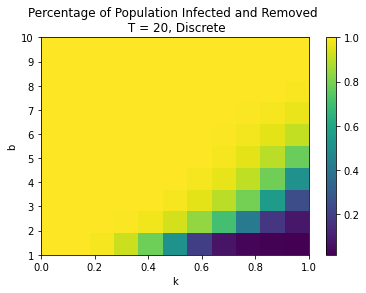
\includegraphics[width=.3\textwidth]{Figure1_discrete_diagT20total.png}\hfill
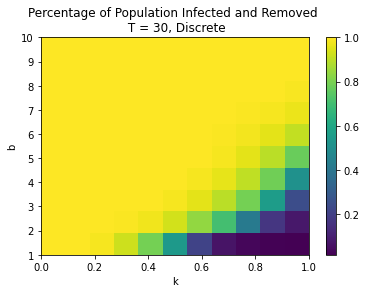
\includegraphics[width=.3\textwidth]{Figure1_discrete_diagT30total.png}

\caption{Phase diagrams for total percentage of population infected (i+r), discrete}
\label{fig:figure3}

\end{figure}



In figure 3, three phase diagrams illustrate the percentage of population infected and removed, i.e., the total percentage of population infected. It depends on both b, the number of interactions per day per individual that could spread the disease, and k, the recovery rate. The diagrams look very similar for different lengths of simulation (10, 20, and 30 days). It is clear that as k increases and b decreases, the total percentage of population infected decreases. If each individual only has less than two interactions per day that could spread the disease and the recovery rate is higher than 0.6, then almost nobody will be infected over time. The yellow area represents that everyone is eventually infected. When k is less or equal to 0.2, then everyone is eventually infected. Also, when b is larger than 6, everyone is eventually infected. Furthermore, when b is relatively small (less than 7) but k is relatively large (larger than 0.3), everyone is eventually infected. More precisely, the cut edge between the area where all individuals are infected and the remaining area is approximately linear, so that we may estimate the edge by $b = 10k - 3$. Therefore, when $b - 10k + 3 > 0$, everyone is eventually infected. 

\begin{figure}[htp]

\centering
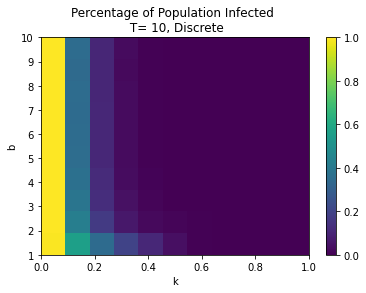
\includegraphics[width=.3\textwidth]{Figure1_discrete_diagT10infect.png}\hfill
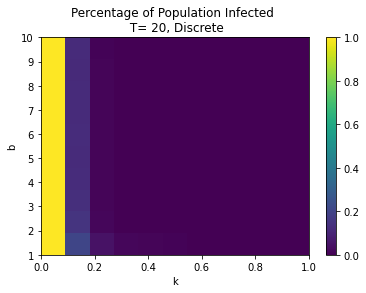
\includegraphics[width=.3\textwidth]{Figure1_discrete_diagT20infect.png}\hfill
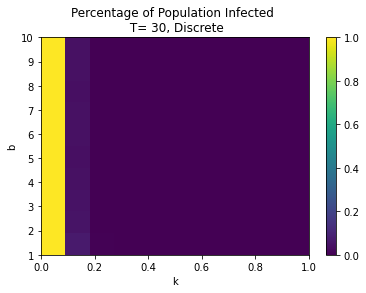
\includegraphics[width=.3\textwidth]{Figure1_discrete_diagT30infect.png}

\caption{Phase diagrams for percentage of population infected (i), discrete}
\label{fig:figure3}

\end{figure}



Then, we try to discover the parameter regimes that i will quickly go to 0. Figure 4 shows the phase diagrams for only infected population. We conclude that the percentage of infected people will quickly goes to 0, if the recovery rate k is large. Specifically, our simulations demonstrate when k is larger than 0.3, i will quickly go to 0 regardless of b. 


\subsection{Continuous/ODE-Based Model}




\section{Part 4}
\subsection{Modelling the usage of mask}
Although it is now recommended and a common practice to wear mask to limit the spread of COVID 19, it is very controversial at the beginning of the pandemic that whether it is neccesary and efficient to wear mask. In this variation, we will study how the use of mask will influence the percentage of deaths and hospitalizations with respect to different infectious contact rate. The model is based on the paper "To mask or not to mask: Modeling the potential for face mask
use by the general public to curtail the COVID-19 pandemic" by Steffen E. Eikenberry et al.
In this model, we will introduce seven varaibles. S(t),E(t),I(t),H(t),A(t),R(t) each denote susceptible, exposed, symptomatic infectious, hospitalized, asymptomatic infectious, and recovered classes, with an assumption that people progress from \\
S $\rightarrow$ E $\rightarrow$ A $\rightarrow$ I $\rightarrow$H \\ At each state, infectious people will be able to recover, and only people in severe condition will go to hosptial and may die.\\D(t) is also included to track cumulative deaths. Two sets of ODE euqations will be used during simulation to find how use of mask will impact the spread of disease. We first consider a baseline model for the case where no masks are used. In the second set of odes, we will introduce more variables
$S_{U}(t)$,$E_{U}(t)$,$I_{U}(t)$,$H_{U}(t)$,$A_{U}(t)$,$R_{U}(t)$,$S_{M}(t)$,$E_{M}(t)$,$I_{M}(t)$,$H_{M}(t)$,$A_{M}(t)$,$R_{M}(t)$ to divide the population in two part: The population wearing masks and the one not wearing masks
Here are two sets of Odes:\\
\begin{minipage}{0.45\textwidth}
\begin{eqnarray}
  \frac{dS}{dt} &=& -\beta{(t)}(I+\eta A)\frac{S}{N}\nonumber\\
  \frac{dE}{dt} &=& \beta(t)(I+\eta A)\frac{S}{N}-\sigma{E}\nonumber\\
  \frac{dI}{dt} &=& \alpha\sigma{E}-\phi{I}-\gamma_{I}I\nonumber\\
  \frac{dA}{dt} &=& (1-\alpha)\sigma E-\gamma_{A}A\nonumber\\
  \frac{dH}{dt} &=& \phi I - \sigma H - \gamma_{H}H\nonumber\\
  \frac{dR}{dt} &=& \gamma_{I}{I} + \gamma_{A}{A}+\gamma_{H}{H}\nonumber\\
  \frac{dD}{dt} &=& \sigma H\nonumber\\
\end{eqnarray}
\end{minipage}
\begin{minipage}{0.35\textwidth}
\small
\begin{eqnarray}
  \frac{dS_{U}}{dt} &=& -\beta(I_{U}+\eta A_{U})\frac{S_{U}}{N}-\beta((1-\epsilon_{0})I_{M}+(1-\epsilon_{0})\eta A_{M})\frac{S_{U}}{N}\nonumber\\
  \frac{dE_{U}}{dt} &=& \beta(I_{U}+\eta{A}_{U})\frac{S_{U}}{N}+\beta((1-\epsilon_{0})I_{M}+(1-\epsilon_{0})\eta A_{M}))\frac{S_{U}}{N}-\sigma E_{U}\nonumber\\
  \end{eqnarray}
\end{minipage}

We will run the simulation and observe what will happen in several days. \\Here,$\beta$ is the infectious contact rate, $\sigma$ is the transition exposed to infectious\\$\eta$ is the infectiousness factor for asymptomatic carriar, $\alpha$ is the fraction of infections that become symptomatic\\
$\phi$ is rate of hospitalization,$\gamma_{A}$ is the recovery rate for asymptomatic
\\$\gamma_{I}$ is the recovery rate, symptomatic,$\gamma_{H}$ is the recovery rate for hospitalized.\\$\sigma$ is the death rate in hospital.$\epsilon_{0}$ is the outward efficiency of the masks while $\epsilon_{i}$ is the inward efficiency of the masks.\\

We will find the default estimated values for all parameters with population masked and not masked.
Here, an assumption is made that the inward efficiency and outward efficiency of masks are the same($\epsilon_{0} = \epsilon_{1}$. We will draw a 2 dimensional phase diagram to show how the efficiency of mask(homemade mask or surgery mask) and the percentage of masked people will influence the hospitalization as well as the total deaths among the population. 


\subsection{Fitting the data with SIR model}




\end{document}

